\documentclass[22pt]{beamer}
\usepackage[orientation=portrait, size=custom, width=90.44, height=65,scale=1.2]{beamerposter} % 36in*2.5 = 90cm
\usepackage[absolute,overlay]{textpos}
\usepackage{bookmark} %pdflatex says to use this to avoid errors...
\usepackage{graphicx} %for including images
\graphicspath{{figs/}} %location of images
\usepackage{wrapfig} %wrap text around the images
\usepackage{listingsutf8}    %package for code environment; use this instead of verbatim to get automatic line break; use this instead of listings to get (•)
\usepackage{amsmath}
\usepackage{gensymb}
\usepackage[export]{adjustbox}
\usepackage[skins,theorems]{tcolorbox}
\usepackage{pgfplots}
\usepackage{tikz}
\usetikzlibrary{datavisualization}
\usetikzlibrary{datavisualization.formats.functions}
\usetikzlibrary{backgrounds}
\newcommand*\circled[1]{\tikz[baseline=(char.base)]{
            \node[shape=circle,draw,inner sep=2pt] (char) {#1};}}
\usepackage{array}
\usepackage{booktabs,adjustbox}
\usepackage{caption}
\captionsetup[figure]{font=scriptsize, labelfont=scriptsize}
\usepackage{ragged2e}
\usepackage{subfig}
\usepackage{xcolor}
\usepackage{scrextend}

\usepackage[english]{babel}
\usepackage{blindtext}

%\mode<presentation>
%this doesn't seem to make any difference; leave for now for trying out
\usetheme{Berlin}
\definecolor{MacBlue}{rgb}{0.10196,0.22353,0.53725}
\definecolor{MacMaroon} {rgb}{0.47843, 0, 0.23137}
\definecolor{MacMaroon2} {rgb}{0.47451, 0, 0}
\definecolor{MacGray}{rgb}{0.50196,0.49804,0.51765}
\definecolor{MacMaroon3}{rgb}{00.47,0.2,0.31}
\definecolor{MacGold}{rgb}{1, 0.75,0.35}
\usecolortheme[named=MacBlue]{structure}
\setbeamertemplate{caption}[numbered]
\setbeamertemplate{navigation symbols}{}
% \setbeamercolor{background canvas}{bg=MacGray}

\title{Hakaru Language: Standard Library Implementation and Language Validation Testing}
\subtitle{}  %probably want a better subtitle
  \author[Justin Staples, Mahmoud Khattab, Nevin Mahilal and Aryan Sohrabi]{Justin Staples, Mahmoud Khattab, Nevin Mahilal and Aryan Sohrabi, supervised by Dr.~Christopher Anand \& Dr.~Jacques Carette \vspace{0.3cm} \newline \small \{staplejw, khattm, mahilank, sohraa3, anandc, carette\}@mcmaster.ca}
  \institute[McMaster University]{\small{Department of Computing and Software, McMaster University}}
  \date{}

\newenvironment{variableblock}[3]{%
  \setbeamercolor{block body}{#2}
  \setbeamercolor{block title}{#3}
  \begin{block}{#1}}{\end{block}}

\begin{document}
%compile with pdflatex

%there is only one frame, because there is only one page; yeah, it's a poster
%textblock and block seem to work nicely to organize layout
\begin{frame}[fragile]

\begin{textblock}{2}(0.8,0.9)

\includegraphics[height=8.5cm]{mac.png}
\end{textblock}

\begin{textblock}{2}(12.9,0.6)
\includegraphics[height=11cm]{fireball.png} 
\end{textblock}

\begin{textblock}{8}(4,1)
\titlepage
\end{textblock}

\begin{textblock}{5}(0.25,3.5)

%%%%%%%%%%%%%%%%%%%%%%%%%%%%%%%%%%%%%%%%%%%%%%%%%%%%%%%%%%%%%%%%%%%%%%
% Introduction
%%%%%%%%%%%%%%%%%%%%%%%%%%%%%%%%%%%%%%%%%%%%%%%%%%%%%%%%%%%%%%%%%%%%%%

\begin{block}{\Large{Introduction}}
\justifying

\small{Hakaru is an experimental \textbf{probabilistic programming language}, which simplifies implementing models of statistical distributions.

\begin{itemize}
    \item Niche application, small language.
    \item Models output a stream of numbers  distributed according to the implemented distribution.
    \item Models can be compiled to C and Haskell for use in larger applications.
\end{itemize}

}

\bigskip
\small{{\tt \small{hk-maple}} is an inference algorithm suite that uses Maple to perform algebraic transformations on Hakaru programs to produce equivalent models with greater sampling efficiency.}

\end{block}

%%%%%%%%%%%%%%%%%%%%%%%%%%%%%%%%%%%%%%%%%%%%%%%%%%%%%%%%%%%%%%%%%%%%%%
% Motivation
%%%%%%%%%%%%%%%%%%%%%%%%%%%%%%%%%%%%%%%%%%%%%%%%%%%%%%%%%%%%%%%%%%%%%%

\begin{block}{\Large{Motivation}}
\justifying

\small{Increase language accessibility:
\begin{itemize}
  \item Standard Library Development: focus on univariate distributions.
  \item Added in primitive math functions that were incomplete (log(x)) or missing (choose(n,k)). 
  \item Syntax-highlighting-for-hakaru package for Sublime Text (Figures 2 and 3).
\end{itemize}
}

\bigskip
\small{Test language validity: 
\begin{itemize}
  \item Use known relationships between distributions to test the validity of program transformations like {\tt \small{hk-maple}}.
\end{itemize} }
\justifying


\end{block}


%%%%%%%%%%%%%%%%%%%%%%%%%%%%%%%%%%%%%%%%%%%%%%%%%%%%%%%%%%%%%%%%%%%%%%
% Key Concepts
%%%%%%%%%%%%%%%%%%%%%%%%%%%%%%%%%%%%%%%%%%%%%%%%%%%%%%%%%%%%%%%%%%%%%%

\begin{block}{\Large{Key Concepts}}
\justifying

\small{
\begin{itemize}
  \item[\textbf{$\star$}] \textit{PDF: Probability Density.}
  \item[\textbf{$\star$}] \textit{UDR chart: Univariate Distribution Relationship chart.}
  \item[\textbf{$\star$}] `{\textbf{$\sim$}}' vs `{\textbf{$<\sim$}}':
      \begin{itemize}
          \small
          \item[--] \small{$X \sim Normal(0, 1)$: random variable, $X$, is distributed according to a normal distribution (statistics literature).}
          \item[--] \small{{\tt \small{x $<\sim$ normal(0, 1)}}: pull a random sample from a normal distribution and bind it {\tt \small{x}} (Hakaru code).}
      \end{itemize}

\end{itemize}
}
\end{block}

\begin{block}{\Large{Standard Library Development}}

\small{The Standard Library implements commonly used univariate distributions. We have followed the UDR to implement distributions with the following guiding principles:


\small{

\bigskip
\begin{itemize}
  \item When possible, implement distributions as transformations on pre-existing models.
  \item In case of many possible implementations, take the shortest path from a primitive distribution on the UDR.
\end{itemize}
        }
}

\end{block}


\begin{textblock}{5}(5.5,3.5)




%%%%%%%%%%%%%%%%%%%%%%%%%%%%%%%%%%%%%%%%%%%%%%%%%%%%%%%%%%%%%%%%%%%%%%
% Standard Library Development
%%%%%%%%%%%%%%%%%%%%%%%%%%%%%%%%%%%%%%%%%%%%%%%%%%%%%%%%%%%%%%%%%%%%%%

\begin{variableblock}{}{}{}
\justifying



\bigskip

\begin{figure}
\centering
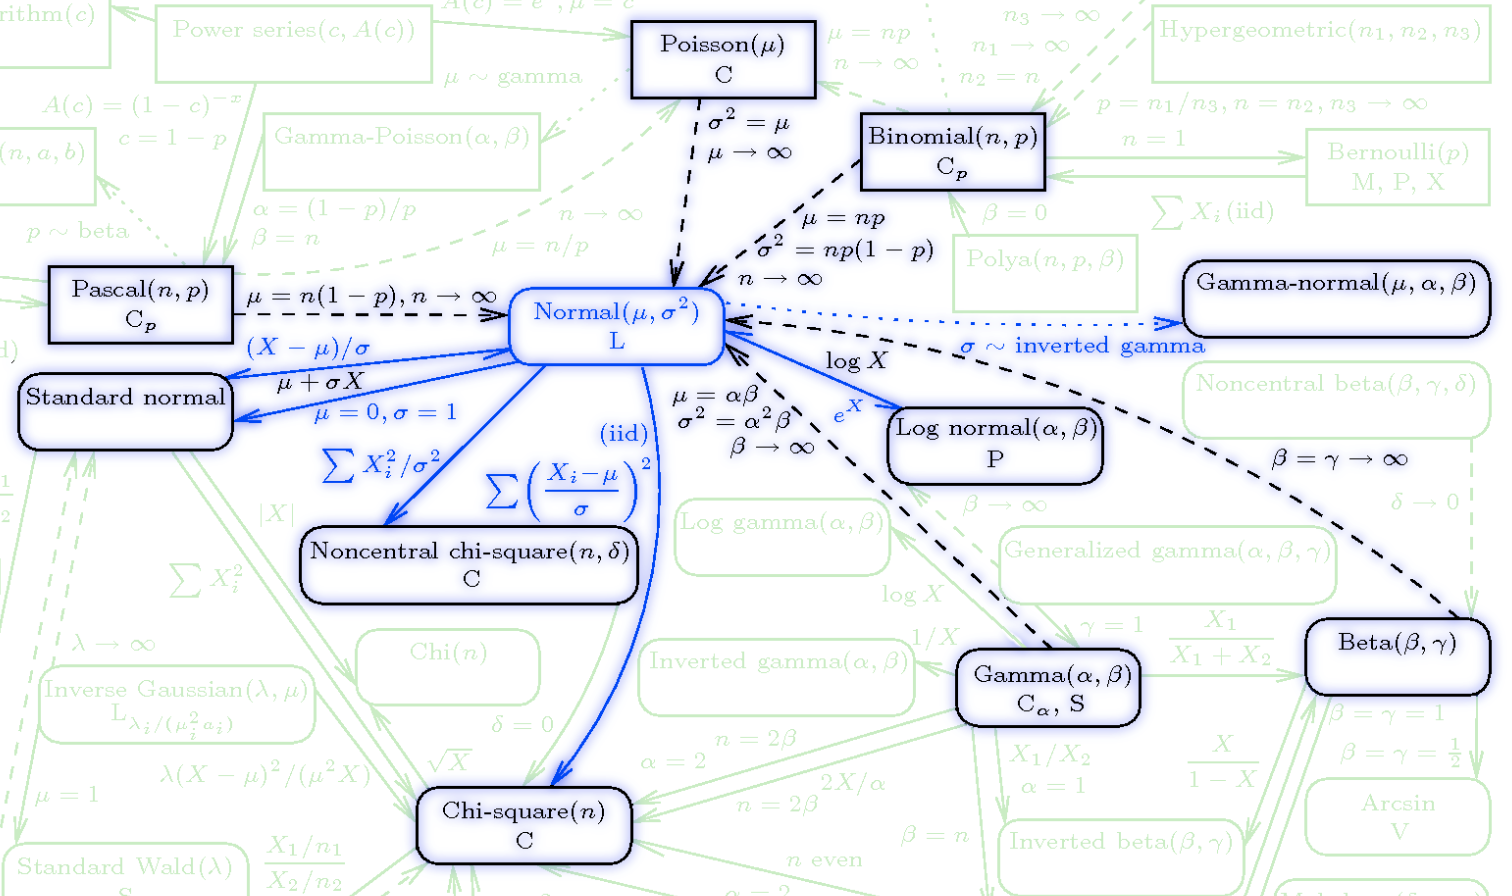
\includegraphics[height=10.7cm]{UDR.png}
\caption{\tiny{A snapshot of the UDR $^{[1]}$ shows how the normal distribution can be transformed into a multitude of other distributions.}}
\end{figure}

\small{Hakaru does not allow us to transform models directly. Must apply transformations to samples pulled from the model using the bind {\tt \tiny{<$\sim$}} operator. Therefore, we are interested in implementing transformations of the form:}

\begin{equation*}
\begin{aligned}
& \tcboxmath[boxrule=2pt,colframe=MacMaroon]{R(p, q) \Rightarrow \textit{X} \sim A(p) \Rightarrow \textit{f(X)} \sim B(q)}
\end{aligned}
\end{equation*}

\bigskip

\small We can extend this definition to include transformations defined in terms of an aggregation of many independent samples. For example, the standard chi-square distribution is defined as the sum of the squares of \textit{n} normal random variables (see Figure 2). 

\bigskip
\begin{figure}
\centering
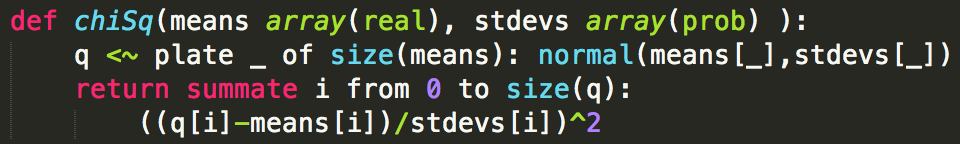
\includegraphics[height=3cm]{chi-square.png}
\caption{\tiny{Our implementation of the chi-square distribution.}}
\end{figure}

\bigskip
\small{Hakaru also lends itself well to Bayesian transformations, which take the following form. The gamma-poisson distribution can be described by such a transformation (see Figure 3).}

\begin{equation*}
\begin{aligned}
& \tcboxmath[boxrule=2pt,colframe=MacMaroon]{X \sim A(p) \Rightarrow Y \sim B(q, X) = C(p, q)}
\end{aligned}
\end{equation*}

~
~
~

\begin{figure}
\centering
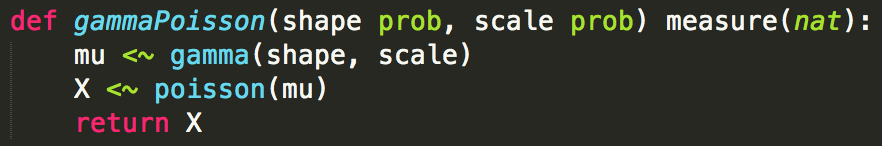
\includegraphics[height=3cm]{gamma-poisson.png}
\caption{\tiny{Our implementation of the gamma-poisson distribution.}}
\end{figure}

\small{In the case of unreachable distributions, we have implemented models in terms of their PDF.}

\bigskip
\small{

Plotting a histogram of a sample population drawn from a model and comparing its shape to that of its PDF, we can have some confidence that an implementation is correct.

}

\end{variableblock}



\end{textblock}

\end{textblock}


\begin{textblock}{5}(10.75,3.5)

\begin{variableblock}{}{}{}
\justifying

\begin{figure}[!tbp]
  \centering
  \subfloat[]{ 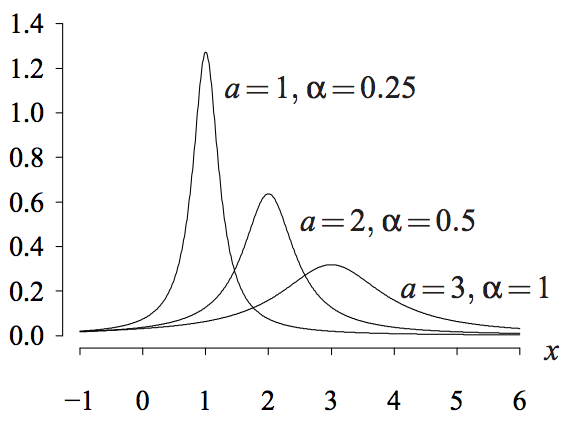
\includegraphics[width=0.38\textwidth]{cauchy.png}\label{fig:f1}}
  \subfloat[]{ 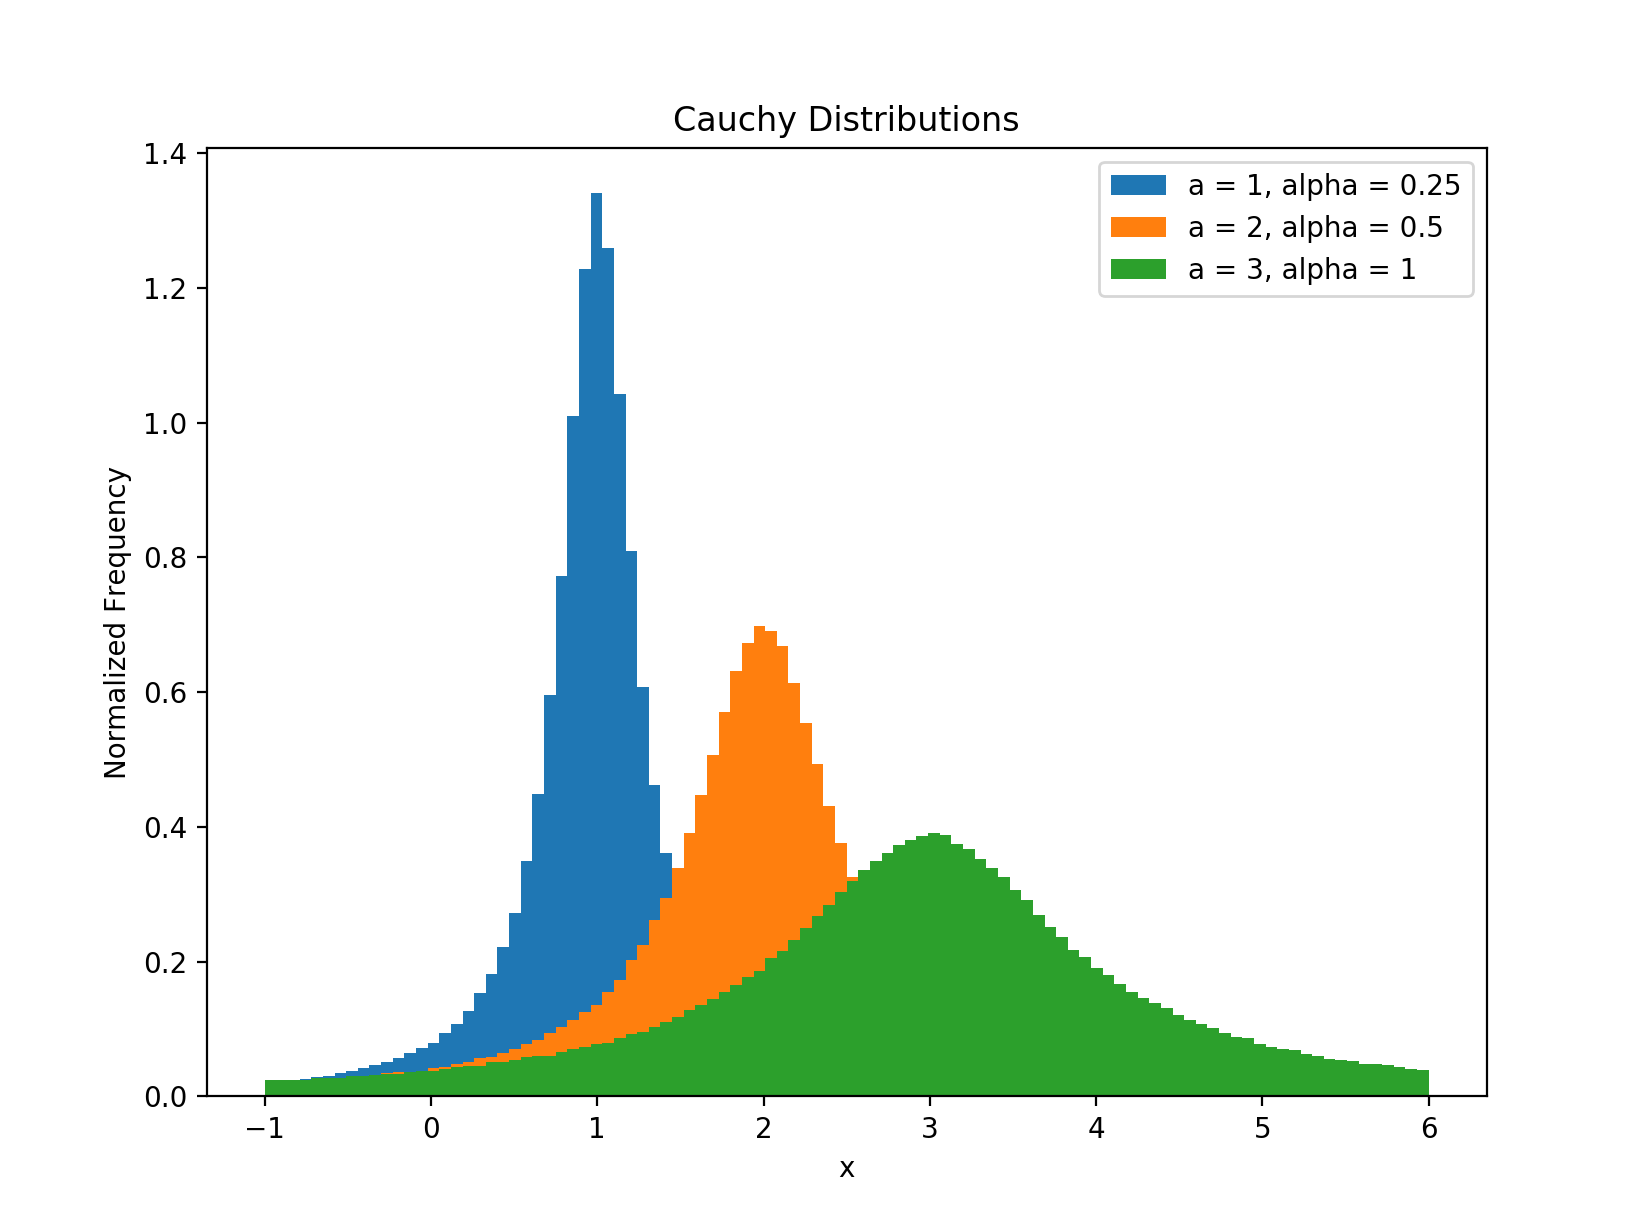
\includegraphics[width=0.38\textwidth]{cauchy_2.png}\label{fig:f2}}
  \caption{\tiny{A few plots of the Cauchy distribution are shown $^{[1]}$, along with a few histograms of data that have been sampled from a Hakaru program.}}
\end{figure}


\end{variableblock}

%%%%%%%%%%%%%%%%%%%%%%%%%%%%%%%%%%%%%%%%%%%%%%%%%%%%%%%%%%%%%%%%%%%%%%
% Testing Relationships Between Distributions
%%%%%%%%%%%%%%%%%%%%%%%%%%%%%%%%%%%%%%%%%%%%%%%%%%%%%%%%%%%%%%%%%%%%%%

\begin{block}{\Large{Testing Relationships Between Distributions}}
\justifying


\small{Hakaru's validity can be tested by checking if it recognizes known relationships between distributions. More specifically:

\bigskip


\begin{addmargin}[2em]{2em}
\textit{Hypothesis: By applying appropriate transformations to implementations of distributions, A and B, we can create two distinct Hakaru programs which, when passed to {\tt \small{hk-maple}}, will reduce to equivalent Hakaru code.}
\end{addmargin}

\bigskip
Test cases are written in Hakaru, therefore we test relationships of the forms discussed. There are hundreds of possible tests. We have focused on a small set of distributions.

\bigskip
Almost all test cases failed. These failures could be due to an error in the language implementation, or a bug in one of the {\tt \small{hk-maple}} algorithms. Sometimes tests fail as a consequence of intended design choice. These failures give the language developers useful information for continuing to make Hakaru more robust.
}

\end{block}

%%%%%%%%%%%%%%%%%%%%%%%%%%%%%%%%%%%%%%%%%%%%%%%%%%%%%%%%%%%%%%%%%%%%%%
% Conclusions & Future Work
%%%%%%%%%%%%%%%%%%%%%%%%%%%%%%%%%%%%%%%%%%%%%%%%%%%%%%%%%%%%%%%%%%%%%%

\begin{block}{\Large{Conclusions \& Future Work}}

\small{The project was successful in increasing language accessibility, both in terms of Standard Library Development and filled in language features. Testing has proven there is still a lot of work to be done. Here are some suggestions for future work:

\begin{itemize}
    \item Languages Features: Hakaru needs import and error/exception handling. 
    \item Stdlib Dev: multivariate distributions
    \item Testing: hundreds of known relationships untested 
\end{itemize}

}

\end{block}

%%%%%%%%%%%%%%%%%%%%%%%%%%%%%%%%%%%%%%%%%%%%%%%%%%%%%%%%%%%%%%%%%%%%%%
% References
%%%%%%%%%%%%%%%%%%%%%%%%%%%%%%%%%%%%%%%%%%%%%%%%%%%%%%%%%%%%%%%%%%%%%%

\begin{block}{\Large{References}}

\small{[1]~L. Leemis, "Univariate Distribution Relationship Chart", Math.wm.edu, 2018. [Online]. Available: http://www.math.wm.edu/~leemis/chart/UDR/UDR.html. 

[2]~P. Narayanan, J. Carette, W. Romano, C. Shan and R. Zinkov, “Probabilistic Inference by Program Transformation in Hakaru (System Defootnoteion)”, Functional and Logic Programming, pp. 62-79, 2016.}


\end{block}


% \begin{block}{References}
% \setbeamertemplate{bibliography item}{\insertbiblabel}
% \bibliographystyle{ieeetr}
% {\size
% \bibliography{../bib}}
% \end{block}

\end{textblock}
\end{frame}
\end{document}
